\chapter{Specifikacija programske potpore}

\section{Funkcionalni zahtjevi}

\noindent \textbf{Dionici:}

\begin{packed_enum}

\item Studenti
\item Profesori
\item Asistenti
\item Sveučilište u Zagrebu
\item Razvojni tim

\end{packed_enum}

\noindent \textbf{Aktori i njihovi funkcionalni zahtjevi:}

\begin{packed_enum}
\item  \underbar{Anonimni korisnik (inicijator) može:}

    \begin{packed_enum}

    \item prijaviti se u aplikaciju
    \item stvoriti profil
    \item pretraživati članke
        \begin{packed_enum}

        \item po kategorijama
        \item po naslovu

        \end{packed_enum}
    \item vidjeti određeni članak
    \item podijeliti članak na društvenim mrežama
    \item pregledati tuđe profile

    \end{packed_enum}

\item  \underbar{Prijavljeni korisnik (inicijator) može:}

    \begin{packed_enum}

    \item se odjaviti
    \item stvoriti

        \begin{packed_enum}

        \item članak
        \item komentar na članak

        \end{packed_enum}

    \item urediti

        \begin{packed_enum}

        \item svoj članak
        \item svoj komentar na članak
        \item svoj profil

        \end{packed_enum}

    \item obrisati

        \begin{packed_enum}

        \item svoj članak
        \item svoj komentar na članak

        \end{packed_enum}

    \item vidjeti obavijesti
    \item ocijeniti tuđi članak
    \item pregledati svoj profil
    \item obrisati svoj profil
    \item prijaviti članak

    \end{packed_enum}

\item \underbar{Moderator (inicijator) može:}

    \begin{packed_enum}

    \item zatražiti izmjenu članka
    \item zatražiti izmjenu komentara
    \item obrisati tuđi članak
    \item orisati tuđi komentar
    \item slati obavijesti
    \item privremeno/trajno banati korisnika

    \end{packed_enum}

\item \underbar{Administrator (inicijator) može:}

    \begin{packed_enum}

    \item dodati moderatora/administratora
    \item ukloniti moderatora
    \item odstupiti s mjesta administratora

    \end{packed_enum}

\end{packed_enum}

\eject 

\subsection{Obrasci uporabe}

\subsubsection{Opis obrazaca uporabe}

\noindent \underbar{\textbf{UC1 - Prijava u aplikaciju}}
\begin{packed_item}

\item \textbf{Glavni sudionik:} Anonimni korisnik
\item  \textbf{Cilj:} Prijaviti se u aplikaciju
\item  \textbf{Sudionici:} Baza podataka
\item  \textbf{Preduvjet:} Korisnik je registriran
\item  \textbf{Opis osnovnog tijeka:}

\item[] \begin{packed_enum}

    \item Korisnik ulazi u sučelje za prijavu
    \item Korisnik unosi email adresu i šifru
    \item Provjera valjanosti podataka
    \item Korisnik ulazi u aplikaciju kao prijavljeni korisnik

\end{packed_enum}

\item  \textbf{Opis mogućih odstupanja:}

\item[] \begin{packed_item}

    \item[3.a] Unesena je neispravna email adresa ili šifra

    \item[] \begin{packed_enum}

        \item Sustav obavještava korisnika o neispravnosti unesenih podataka, i predlaže korisniku promjenu unesenih podataka

    \end{packed_enum}

\end{packed_item}

\end{packed_item}

\noindent \underbar{\textbf{UC2 - Stvaranje računa}}
\begin{packed_item}

\item \textbf{Glavni sudionik:} Anonimni korisnik
\item  \textbf{Cilj:} Stvoriti račun
\item  \textbf{Sudionici:} Baza podataka
\item  \textbf{Preduvjet:} -
\item  \textbf{Opis osnovnog tijeka:}

\item[] \begin{packed_enum}

    \item Korisnik ulazi u sučelje za stvaranje računa
    \item Korisnik unosi ime, email adresu i šifru
    \item Provjera valjanosti podataka
    \item Sustav dojavljuje korisniku kako je registracija uspješna

\end{packed_enum}

\item  \textbf{Opis mogućih odstupanja:}

\item[] \begin{packed_item}

    \item[3.a] Račun s već navedenom email adresom već postoji

    \item[] \begin{packed_enum}

        \item Sustav predlaže korisniku promjenu unesene email adrese ili prijavu u postojeći profil pod navedenom adresom

    \end{packed_enum}

\item[3.b] Šifra je preslaba

\item[] \begin{packed_enum}

    \item Sustav predlaže korisniku promjenu unesene šifre

\end{packed_enum}

    \item[3.c] Drugi unos šifre se ne podudara s prvim

    \item[] \begin{packed_enum}

        \item Sustav obavještava korisnika da se šifre razlikuju

    \end{packed_enum}

\end{packed_item}

\end{packed_item}

\noindent \underbar{\textbf{UC3 - Pretraga članaka po kategorijama}}
\begin{packed_item}

\item \textbf{Glavni sudionik:} Anonimni/prijavljeni korisnik
\item  \textbf{Cilj:} Pretražiti članke po kategorijama
\item  \textbf{Sudionici:} Baza podataka
\item  \textbf{Preduvjet:} -
\item  \textbf{Opis osnovnog tijeka:}

\item[] \begin{packed_enum}

    \item Korisnik bira kategorije za pretragu
    \item Baza podataka dohvaća članke sa zadanim kategorijama
    \item Korisniku se prikazuju dohvaćeni članci

\end{packed_enum}

\item  \textbf{Opis mogućih odstupanja:}

\item[] \begin{packed_item}

    \item[2.a] U bazi podataka ne postoji članak sa navedenim kategorijama

    \item[] \begin{packed_enum}

        \item Sustav obavještava korisnika da nije dohvaćen niti jedan članak, te da proba suziti izbor kategorija

    \end{packed_enum}

\end{packed_item}

\end{packed_item}

\noindent \underbar{\textbf{UC4 - Pretraga članaka po naslovu}}
\begin{packed_item}

\item \textbf{Glavni sudionik:} Anonimni/prijavljeni korisnik
\item  \textbf{Cilj:} Pretražiti članke po naslovu
\item  \textbf{Sudionici:} Baza podataka
\item  \textbf{Preduvjet:} -
\item  \textbf{Opis osnovnog tijeka:}

\item[] \begin{packed_enum}

    \item Korisnik unosi tekst za pretragu
    \item Baza podataka dohvaća članke koji sadrže zadani tekst u naslovu
    \item Korisniku se prikazuju dohvaćeni članci

\end{packed_enum}

\item  \textbf{Opis mogućih odstupanja:}

\item[] \begin{packed_item}

    \item[2.a] U bazi podataka ne postoji članak sa danim tekstom u naslovu

    \item[] \begin{packed_enum}

        \item Sustav obavještava korisnika da nije dohvaćen niti jedan članak, te da proba promijeniti tekst za pretragu

    \end{packed_enum}

\end{packed_item}

\end{packed_item}

\noindent \underbar{\textbf{UC5 - Pregledavanje članka}}
\begin{packed_item}

\item \textbf{Glavni sudionik:} Anonimni/prijavljeni korisnik
\item  \textbf{Cilj:} Pregledati određeni članak
\item  \textbf{Sudionici:} Baza podataka
\item  \textbf{Preduvjet:} -
\item  \textbf{Opis osnovnog tijeka:}

\item[] \begin{packed_enum}

    \item Dohvaćanje članka sa baze podataka
    \item Prikaz članka na sučelju

\end{packed_enum}

\end{packed_item}

\noindent \underbar{\textbf{UC6 - Dijeljenje članaka}}
\begin{packed_item}

\item \textbf{Glavni sudionik:} Anonimni/prijavljeni korisnik
\item  \textbf{Cilj:} Podijeliti članak na društvenim mrežama
\item  \textbf{Sudionici:} -
\item  \textbf{Preduvjet:} -
\item  \textbf{Opis osnovnog tijeka:}

\item[] \begin{packed_enum}

    \item Korisnik bira opciju za dijeljenje članka
    \item Korisniku se prikazuje izbornik za društvene mreže
    \item Preusmjeravanje na izabranu društvenu mrežu ili kopiranje adrese u korisnikov međuspremnik

\end{packed_enum}

\item  \textbf{Opis mogućih odstupanja:}

\end{packed_item}

\noindent \underbar{\textbf{UC7 - Pregled profila}}
\begin{packed_item}

\item \textbf{Glavni sudionik:} Anonimni/prijavljeni korisnik
\item  \textbf{Cilj:} Pregledati tuđi profil
\item  \textbf{Sudionici:} Baza podataka
\item  \textbf{Preduvjet:} -
\item  \textbf{Opis osnovnog tijeka:}

\item[] \begin{packed_enum}

    \item Korisnik ulazi na stranicu profila
    \item Baza podataka dohvaća javne podatake profila
    \item Korisniku se prikazuju dohvaćeni podaci profila

\end{packed_enum}

\item  \textbf{Opis mogućih odstupanja:}

\item[] \begin{packed_item}

    \item[2.a] Profil ne postoji, ili je izbrisan

    \item[] \begin{packed_enum}

        \item Korisnik se preusmjerava na matičnu stranicu, sa dojavom da profil ne postoji

    \end{packed_enum}

\end{packed_item}

\end{packed_item}

\noindent \underbar{\textbf{UC8 - Odjava sa aplikacije}}
\begin{packed_item}

\item \textbf{Glavni sudionik:} Prijavljeni korisnik
\item  \textbf{Cilj:} Odjaviti se sa aplikacije
\item  \textbf{Sudionici:} Baza podataka
\item  \textbf{Preduvjet:} Korisnik je prijavljen
\item  \textbf{Opis osnovnog tijeka:}

\item[] \begin{packed_enum}

    \item Korisnik bira opciju za odjavu iz aplikacije
    \item Baza podataka briše zapis o prijavi
    \item Korisnik se preusmjerava na stranicu za anonimnog korisnika

\end{packed_enum}

\end{packed_item}

\noindent \underbar{\textbf{UC9 - Stvaranje članaka}}
\begin{packed_item}

\item \textbf{Glavni sudionik:} Prijavljeni korisnik
\item  \textbf{Cilj:} Stvoriti novi članak
\item  \textbf{Sudionici:} Baza podataka
\item  \textbf{Preduvjet:} Korisnik je prijavljen, korisnik nema ograničen pristup
\item  \textbf{Opis osnovnog tijeka:}

\item[] \begin{packed_enum}

    \item Korisnik otvara sučelje za pisanje članka
    \item Korisnik upisuje tekst članka
    \item Korisnik objavljuje članak
    \item Baza podataka sprema članak
    \item Sustav dojavljuje korisniku da je članak objavljen

\end{packed_enum}

\item  \textbf{Opis mogućih odstupanja:}

\item[] \begin{packed_item}

    \item[3.a] Uneseni tekst je prazan

    \item[] \begin{packed_enum}

        \item Sustav dojavljuje korisniku da tekst ne smije biti prazan

    \end{packed_enum}

\end{packed_item}

\end{packed_item}

\noindent \underbar{\textbf{UC10 - Uređivanje članaka}}
\begin{packed_item}

\item \textbf{Glavni sudionik:} Prijavljeni korisnik
\item  \textbf{Cilj:} Urediti vlastiti članak
\item  \textbf{Sudionici:} Baza podataka
\item  \textbf{Preduvjet:} Korisnik je prijavljen, članak pripada korisniku
\item  \textbf{Opis osnovnog tijeka:}

\item[] \begin{packed_enum}

    \item Korisnik bira opciju za uređivanje članka
    \item Otvara se sučelje za pisanje članka
    \item Korisnik unosi promjene u članak
    \item Korisnik objavljuje članak
    \item Baza podataka sprema promjene članka
    \item Sustav dojavljuje korisniku da je članak uređen

\end{packed_enum}

\item  \textbf{Opis mogućih odstupanja:}

\item[] \begin{packed_item}

    \item[3.a] Članak je prazan/nepromijenjen

    \item[] \begin{packed_enum}

        \item Sustav dojavljuje korisniku da tekst ne smije biti prazan/nepromijenjen

    \end{packed_enum}

\end{packed_item}

\end{packed_item}

\noindent \underbar{\textbf{UC11 - Brisanje vlastitog članka}}
\begin{packed_item}

\item \textbf{Glavni sudionik:} Prijavljeni korisnik
\item  \textbf{Cilj:} Obrisati vlastiti članak
\item  \textbf{Sudionici:} Baza podataka
\item  \textbf{Preduvjet:} Korisnik je prijavljen, članak pripada korisniku
\item  \textbf{Opis osnovnog tijeka:}

\item[] \begin{packed_enum}

    \item Korisnik bira opciju za brisanje članka
    \item Otvara se sučelje za potvrdu brisanja članka
    \item Korisnik potvrđuje brisanje članka
    \item Baza podataka briše članak

\end{packed_enum}

\item  \textbf{Opis mogućih odstupanja:}

\item[] \begin{packed_item}

    \item[3.a] Korisnik nije potvrdio brisanje članka
    \item[] \begin{packed_enum}

        \item Članak se ne briše

    \end{packed_enum}

\end{packed_item}
\end{packed_item}

\noindent \underbar{\textbf{UC12 - Pregled obavijesti}}
\begin{packed_item}

\item \textbf{Glavni sudionik:} Prijavljeni korisnik
\item  \textbf{Cilj:} Pregledati obavijesti
\item  \textbf{Sudionici:} Baza podataka
\item  \textbf{Preduvjet:} Korisnik je prijavljen
\item  \textbf{Opis osnovnog tijeka:}

\item[] \begin{packed_enum}

    \item Korisnik otvara sučelje za prikaz obavijesti
    \item Baza podataka dohvaća obavijesti

\end{packed_enum}

\item  \textbf{Opis mogućih odstupanja:}

\item[] \begin{packed_item}

    \item[2.a] Nema zapisa o obavijestima za korisnika
    \item[] \begin{packed_enum}

        \item Sustav dojavljuje korisniku da nema obavijesti

    \end{packed_enum}

\end{packed_item}
\end{packed_item}

\noindent \underbar{\textbf{UC13 - Ocjenjivanje članaka}}
\begin{packed_item}

\item \textbf{Glavni sudionik:} Prijavljeni korisnik
\item  \textbf{Cilj:} Ocijeniti tuđi članak
\item  \textbf{Sudionici:} Baza podataka
\item  \textbf{Preduvjet:} Korisnik je prijavljen
\item  \textbf{Opis osnovnog tijeka:}

\item[] \begin{packed_enum}

    \item Korisnik ocjenjuje članak jednom od predodređenih ocjena
    \item Baza podataka sprema zapis o ocjeni od korisnika na članak
    \item Sučelje osvježava prikaz o ocjenama članka

\end{packed_enum}

\item  \textbf{Opis mogućih odstupanja:}

\item[] \begin{packed_item}

    \item[2.a] Korisnik je već ostavio ocjenu na članak
    \item[] \begin{packed_enum}

        \item Baza podataka unosi promjene na već postojeći zapis

    \end{packed_enum}

    \item[2.b] Korisnik pokušava ostaviti ocjenu na vlastiti članak
    \item[] \begin{packed_enum}

        \item Sustav dojavljuje korisniku da ne može ocijeniti vlastiti članak

    \end{packed_enum}

\end{packed_item}
\end{packed_item}

\noindent \underbar{\textbf{UC14 - Komentiranje članaka}}
\begin{packed_item}

\item \textbf{Glavni sudionik:} Prijavljeni korisnik
\item  \textbf{Cilj:} Komentirati članak
\item  \textbf{Sudionici:} Baza podataka
\item  \textbf{Preduvjet:} Korisnik je prijavljen, korisnik nema ograničen pristup
\item  \textbf{Opis osnovnog tijeka:}

\item[] \begin{packed_enum}

    \item Korisnik otvara sučelje za pisanje komentara
    \item Korisnik upisuje komentar
    \item Korisnik objavljuje komentar

\end{packed_enum}

\item  \textbf{Opis mogućih odstupanja:}

\item[] \begin{packed_item}

    \item[3.a] Komentar je prazan
    \item[] \begin{packed_enum}

        \item Sustav dojavljuje korisniku da komentar ne smije biti prazan

    \end{packed_enum}

\end{packed_item}

\end{packed_item}

\noindent \underbar{\textbf{UC15 - Brisanje vlastitih komentara}}
\begin{packed_item}

\item \textbf{Glavni sudionik:} Prijavljeni korisnik
\item  \textbf{Cilj:} Obrisati vlastiti komentar na članak
\item  \textbf{Sudionici:} Baza podataka
\item  \textbf{Preduvjet:} Korisnik je prijavljen, komentar pripada korisniku
\item  \textbf{Opis osnovnog tijeka:}

\item[] \begin{packed_enum}

    \item Korisnik bira opciju za brisanje komentara
    \item Otvara se sučelje za potvrdu brisanja komentara
    \item Korisnik potvrđuje brisanje komentara
    \item Baza podataka briše komentar

\end{packed_enum}

\item  \textbf{Opis mogućih odstupanja:}

\item[] \begin{packed_item}

    \item[3.a] Korisnik nije potvrdio brisanje komentara
    \item[] \begin{packed_enum}

        \item Komentar se ne briše

    \end{packed_enum}

\end{packed_item}
\end{packed_item}

\noindent \underbar{\textbf{UC16 - Pregled vlastitog profila}}
\begin{packed_item}

\item \textbf{Glavni sudionik:} Prijavljeni korisnik
\item  \textbf{Cilj:} Pregledati vlastiti profil
\item  \textbf{Sudionici:} Baza podataka
\item  \textbf{Preduvjet:} Korisnik je prijavljen
\item  \textbf{Opis osnovnog tijeka:}

\item[] \begin{packed_enum}

    \item Korisnik bira opciju za pregled profila
    \item Baza podataka dohvaća podatke profila korisnika
    \item Korisniku se prikazuju dohvaćeni podatci

\end{packed_enum}

\end{packed_item}

\noindent \underbar{\textbf{UC17 - Uređivanje profila}}
\begin{packed_item}

\item \textbf{Glavni sudionik:} Prijavljeni korisnik
\item  \textbf{Cilj:} Urediti vlastiti profil
\item  \textbf{Sudionici:} Baza podataka
\item  \textbf{Preduvjet:} Korisnik je prijavljen
\item  \textbf{Opis osnovnog tijeka:}

\item[] \begin{packed_enum}

    \item Korisnik bira opciju za uređivanje profila
    \item Baza podataka dohvaća trenutne podatke profila korisnika
    \item Korisniku se dohvaćeni podatci prikazuju
    \item Korisnik uređuje podatke
    \item Korisnik sprema promjene profila
    \item Baza podataka sprema promjene profila

\end{packed_enum}

\item  \textbf{Opis mogućih odstupanja:}

\item[] \begin{packed_item}

    \item[6.a] Neki od podataka nisu valjani
    \item[] \begin{packed_enum}

        \item Sustav korisniku dojavljuje da profil nije spremljen, te koji su podatci nevaljani

    \end{packed_enum}

\end{packed_item}
\end{packed_item}

\noindent \underbar{\textbf{UC18 - Brisanje profila}}
\begin{packed_item}

\item \textbf{Glavni sudionik:} Prijavljeni korisnik
\item  \textbf{Cilj:} Izbrisati vlastiti profil
\item  \textbf{Sudionici:} Baza podataka
\item  \textbf{Preduvjet:} Korisnik je prijavljen
\item  \textbf{Opis osnovnog tijeka:}

\item[] \begin{packed_enum}

    \item Korisnik bira opciju za brisanje profila
    \item Otvara se sučelje za potvrdu brisanja profila
    \item Korisnik potvrđuje brisanje profila
    \item Baza podataka briše zapis o korisničkom profilu

\end{packed_enum}

\item  \textbf{Opis mogućih odstupanja:}

\item[] \begin{packed_item}

    \item[3.a] Korisnik nije potvrdio brisanje profila
    \item[] \begin{packed_enum}

        \item Profil se ne briše

    \end{packed_enum}

\end{packed_item}
\end{packed_item}

\noindent \underbar{\textbf{UC19 - Prijavljivanje članaka}}
\begin{packed_item}

\item \textbf{Glavni sudionik:} Prijavljeni korisnik
\item  \textbf{Cilj:} Prijaviti neprimjeren članak
\item  \textbf{Sudionici:} Baza podataka
\item  \textbf{Preduvjet:} Korisnik je prijavljen
\item  \textbf{Opis osnovnog tijeka:}

\item[] \begin{packed_enum}

    \item Korisnik bira opciju za prijavljivanje članka
    \item Korisniku se prikazuje sučelje za opis neprimjerenog sadržaja
    \item Korisnik unosi podatke
    \item Korisnik prijavljuje članak
    \item Baza podataka sprema prijavu članka

\end{packed_enum}

\item  \textbf{Opis mogućih odstupanja:}

\item[] \begin{packed_item}

    \item[5.a] Podatci su neispravni ili nedostaju
    \item[] \begin{packed_enum}

        \item Sustav dojavljuje korisniku da su podatci neispravni ili nedostaju

    \end{packed_enum}

\end{packed_item}
\end{packed_item}

\noindent \underbar{\textbf{UC20 - Pregledavanje komentara}}
\begin{packed_item}

\item \textbf{Glavni sudionik:} Anonimni/prijavljeni korisnik
\item  \textbf{Cilj:} Pregledati komentare na nečiji članak
\item  \textbf{Sudionici:} Baza podataka
\item  \textbf{Preduvjet:} -
\item  \textbf{Opis osnovnog tijeka:}

\item[] \begin{packed_enum}

    \item Korisnik bira opciju za prikaz komentara na članku
    \item Baza podataka dohvaća komentare na članak
    \item Korisniku se prikazuju dohvaćeni komentari

\end{packed_enum}

\item  \textbf{Opis mogućih odstupanja:}

\item[] \begin{packed_item}

    \item[2.a] Na članku nema komentara
    \item[] \begin{packed_enum}

        \item Sustav dojavljuje korisniku da objava nema komentara

    \end{packed_enum}

\end{packed_item}
\end{packed_item}

\noindent \underbar{\textbf{UC21 - Prijavljivanje komentara}}
\begin{packed_item}

\item \textbf{Glavni sudionik:} Prijavljeni korisnik
\item  \textbf{Cilj:} Prijaviti neprimjeren komentar
\item  \textbf{Sudionici:} Baza podataka
\item  \textbf{Preduvjet:} Korisnik je prijavljen
\item  \textbf{Opis osnovnog tijeka:}

\item[] \begin{packed_enum}

    \item Korisnik bira opciju za prijavljivanje komentara
    \item Korisniku se prikazuje sučelje za opis neprimjerenog sadržaja
    \item Korisnik unosi podatke
    \item Korisnik prijavljuje komentar
    \item Baza podataka sprema prijavu komentara

\end{packed_enum}

\item  \textbf{Opis mogućih odstupanja:}

\item[] \begin{packed_item}

    \item[5.a] Podatci su neispravni ili nedostaju
    \item[] \begin{packed_enum}

        \item Sustav dojavljuje korisniku da su podatci neispravni ili nedostaju

    \end{packed_enum}

\end{packed_item}
\end{packed_item}

\noindent \underbar{\textbf{UC22 - Izmjena nečijeg članka}}
\begin{packed_item}

\item \textbf{Glavni sudionik:} Moderator
\item  \textbf{Cilj:} Predložiti drugom korisniku izmjenu članka
\item  \textbf{Sudionici:} Baza podataka, prijavljeni korisnik
\item  \textbf{Preduvjet:} -
\item  \textbf{Opis osnovnog tijeka:}

\item[] \begin{packed_enum}

    \item Moderator bira opciju za izmjenu nečijeg članka
    \item Moderator unosi poruku korisniku i/ili predloženu izmjenu
    \item Moderator šalje obavijest korisniku
    \item Baza podataka stvara zapis obavijesti s porukom za korisnika

\end{packed_enum}

\end{packed_item}

\noindent \underbar{\textbf{UC23 - Izmjena nečijeg komentara}}
\begin{packed_item}

\item \textbf{Glavni sudionik:} Moderator
\item  \textbf{Cilj:} Predložiti drugom korisniku izmjenu komentara
\item  \textbf{Sudionici:} Baza podataka, prijavljeni korisnik
\item  \textbf{Preduvjet:} -
\item  \textbf{Opis osnovnog tijeka:}

\item[] \begin{packed_enum}

    \item Moderator bira opciju za izmjenu nečijeg komentara
    \item Moderator unosi poruku korisniku i/ili predloženu komentara
    \item Moderator šalje obavijest korisniku
    \item Baza podataka stvara zapis obavijesti s porukom za korisnika

\end{packed_enum}

\end{packed_item}

\noindent \underbar{\textbf{UC24 - Brisanje članka}}
\begin{packed_item}

\item \textbf{Glavni sudionik:} Moderator
\item  \textbf{Cilj:} Obrisati članak nekog korisnika
\item  \textbf{Sudionici:} Baza podataka, prijavljeni korisnik
\item  \textbf{Preduvjet:} -
\item  \textbf{Opis osnovnog tijeka:}

\item[] \begin{packed_enum}

    \item Moderator bira opciju za brisanje članka
    \item Moderatoru se prikazuje sučelje za brisanje članka
    \item Moderator unosi dodatne informacije u vezi brisanja članka
    \item Moderator potvrđuje brisanje članka
    \item Baza podataka briše zapis članka i stvara zapis obavijesti o brisanju članka za korisnika

\end{packed_enum}

\item  \textbf{Opis mogućih odstupanja:}

\item[] \begin{packed_item}

    \item[4.a] Moderator nije potvrdio brisanje članka
    \item[] \begin{packed_enum}

        \item Članak se ne briše

    \end{packed_enum}

\end{packed_item}
\end{packed_item}

\noindent \underbar{\textbf{UC25 - Brisanje komentara}}
\begin{packed_item}

\item \textbf{Glavni sudionik:} Moderator
\item  \textbf{Cilj:} Obrisati komentar nekog korisnika
\item  \textbf{Sudionici:} Baza podataka, prijavljeni korisnik
\item  \textbf{Preduvjet:} -
\item  \textbf{Opis osnovnog tijeka:}

\item[] \begin{packed_enum}

    \item Moderator bira opciju za brisanje komentara
    \item Moderatoru se prikazuje sučelje za brisanje komentara
    \item Moderator unosi dodatne informacije u vezi brisanja komentara
    \item Moderator potvrđuje brisanje komentara
    \item Baza podataka briše zapis članka i stvara zapis obavijesti o brisanju komentara za korisnika

\end{packed_enum}

\item  \textbf{Opis mogućih odstupanja:}

\item[] \begin{packed_item}

    \item[4.a] Moderator nije potvrdio brisanje komentara
    \item[] \begin{packed_enum}

        \item Komentar se ne briše

    \end{packed_enum}

\end{packed_item}
\end{packed_item}

\noindent \underbar{\textbf{UC26 - Slanje obavijesti}}
\begin{packed_item}

\item \textbf{Glavni sudionik:} Moderator
\item  \textbf{Cilj:} Poslati obavijest jednom ili više korisnika
\item  \textbf{Sudionici:} Baza podataka, prijavljeni korisnik
\item  \textbf{Preduvjet:} -
\item  \textbf{Opis osnovnog tijeka:}

\item[] \begin{packed_enum}

    \item Moderator bira opciju za slanje obavijesti
    \item Moderatoru se prikazuje sučelje za slanje obavijesti
    \item Moderator unosi grupu korisnika kojoj šalje obavijesti i sadržaj obavijesti
    \item Moderator šalje obavijest korisnicima
    \item U bazi podataka se stvara zapis o obavijesti za sve navedene korisnike

\end{packed_enum}

\item  \textbf{Opis mogućih odstupanja:}

\item[] \begin{packed_item}

    \item[5.a] Jedno od unesenih polja je prazno
    \item[] \begin{packed_enum}

        \item Sustav dojavljuje moderatoru da treba ispuniti prazno polje

    \end{packed_enum}

\end{packed_item}
\end{packed_item}

\noindent \underbar{\textbf{UC27 - Bananje korisnika}}
\begin{packed_item}

\item \textbf{Glavni sudionik:} Moderator
\item  \textbf{Cilj:} Zabraniti pristup korisniku na neke funkcionalnosti aplikacije
\item  \textbf{Sudionici:} Baza podataka, korisnik
\item  \textbf{Preduvjet:} Korisnik nije prethodno dobio ograničenje pristupa
\item  \textbf{Opis osnovnog tijeka:}

\item[] \begin{packed_enum}

    \item Moderator bira opciju za bananje korisnika
    \item Moderatoru se prikazuje sučelje za bananje korisnika
    \item Moderator unosi dodatne informacije o banu
    \item Moderator potvrđuje bananje korisnika
    \item Baza podataka sprema zapis o banu korisnika i obavijesti za korisnika o banu

\end{packed_enum}

\item  \textbf{Opis mogućih odstupanja:}

\item[] \begin{packed_item}

    \item[4.a] Moderator nije potvrdio bananje korisnika
    \item[] \begin{packed_enum}

        \item Korisnik se ne bana

    \end{packed_enum}

\end{packed_item}
\end{packed_item}

\noindent \underbar{\textbf{UC28 - Dodavanje privilegiranog korisnika}}
\begin{packed_item}

\item \textbf{Glavni sudionik:} Administrator
\item  \textbf{Cilj:} Dodati korisnika na mjesto moderatora ili administratora
\item  \textbf{Sudionici:} Baza podataka, prijavljeni korisnik ili moderator
\item  \textbf{Preduvjet:} Korisnik nije prethodno bio privilegiran
\item  \textbf{Opis osnovnog tijeka:}

\item[] \begin{packed_enum}

    \item Administrator bira opciju za promociju korisnika ili moderatora
    \item Administratoru se prikazuje sučelje za promociju korisnika ili moderatora
    \item Administrator bira želi li korisnika promovirati na moderatora i administratora
    \item Administrator potvrđuje promociju
    \item Baza podataka sprema novu poziciju korisnika i zapis o obavijesti o promociji korisnika

\end{packed_enum}

\item  \textbf{Opis mogućih odstupanja:}

\item[] \begin{packed_item}

    \item[4.a] Administrator nije potvrdio promociju korisnika
    \item[] \begin{packed_enum}

        \item Korisniku ostaju iste ovlasti koje je imao

    \end{packed_enum}

\end{packed_item}
\end{packed_item}

\noindent \underbar{\textbf{UC29 - Uklanjanje moderatora}}
\begin{packed_item}

\item \textbf{Glavni sudionik:} Administrator
\item  \textbf{Cilj:} Ukloniti korisniku moderatorske ovlasti
\item  \textbf{Sudionici:} Baza podataka, moderator
\item  \textbf{Preduvjet:} -
\item  \textbf{Opis osnovnog tijeka:}

\item[] \begin{packed_enum}

    \item Administrator bira opciju za uklanjanje moderatora
    \item Administratoru se prikazuje sučelje za potvrdu uklanjanja moderatora
    \item Administrator potvrđuje uklanjanje moderatora
    \item Baza podataka sprema novu poziciju moderatora kao korisnika i zapis o obavijesti gubitka moderatorskih ovlasti

\end{packed_enum}

\item  \textbf{Opis mogućih odstupanja:}

\item[] \begin{packed_item}

    \item[3.a] Administrator nije potvrdio uklanjanje moderatora
    \item[] \begin{packed_enum}

        \item Moderatoru ostaju iste ovlasti koje je imao

    \end{packed_enum}

\end{packed_item}
\end{packed_item}

\noindent \underbar{\textbf{UC30 - Odstupanje s mjesta administratora}}
\begin{packed_item}

\item \textbf{Glavni sudionik:} Administrator
\item  \textbf{Cilj:} Ukloniti sebi administratorske ovlasti
\item  \textbf{Sudionici:} Baza podataka
\item  \textbf{Preduvjet:} -
\item  \textbf{Opis osnovnog tijeka:}

\item[] \begin{packed_enum}

    \item Administrator bira opciju za odstupanje s mjesta administratora
    \item Administratoru se prikazuje sučelje za potvrdu za odstupanje
    \item Administrator potvrđuje odstupanje
    \item Baza podataka sprema novu poziciju administratora

\end{packed_enum}

\item  \textbf{Opis mogućih odstupanja:}

\item[] \begin{packed_item}

    \item[3.a] Administrator nije potvrdio odstupanje
    \item[] \begin{packed_enum}

        \item Administratoru ostaju iste ovlasti koje je imao

    \end{packed_enum}

\end{packed_item}
\end{packed_item}

\subsubsection{Dijagrami obrazaca uporabe}

\begin{figure}[H]
	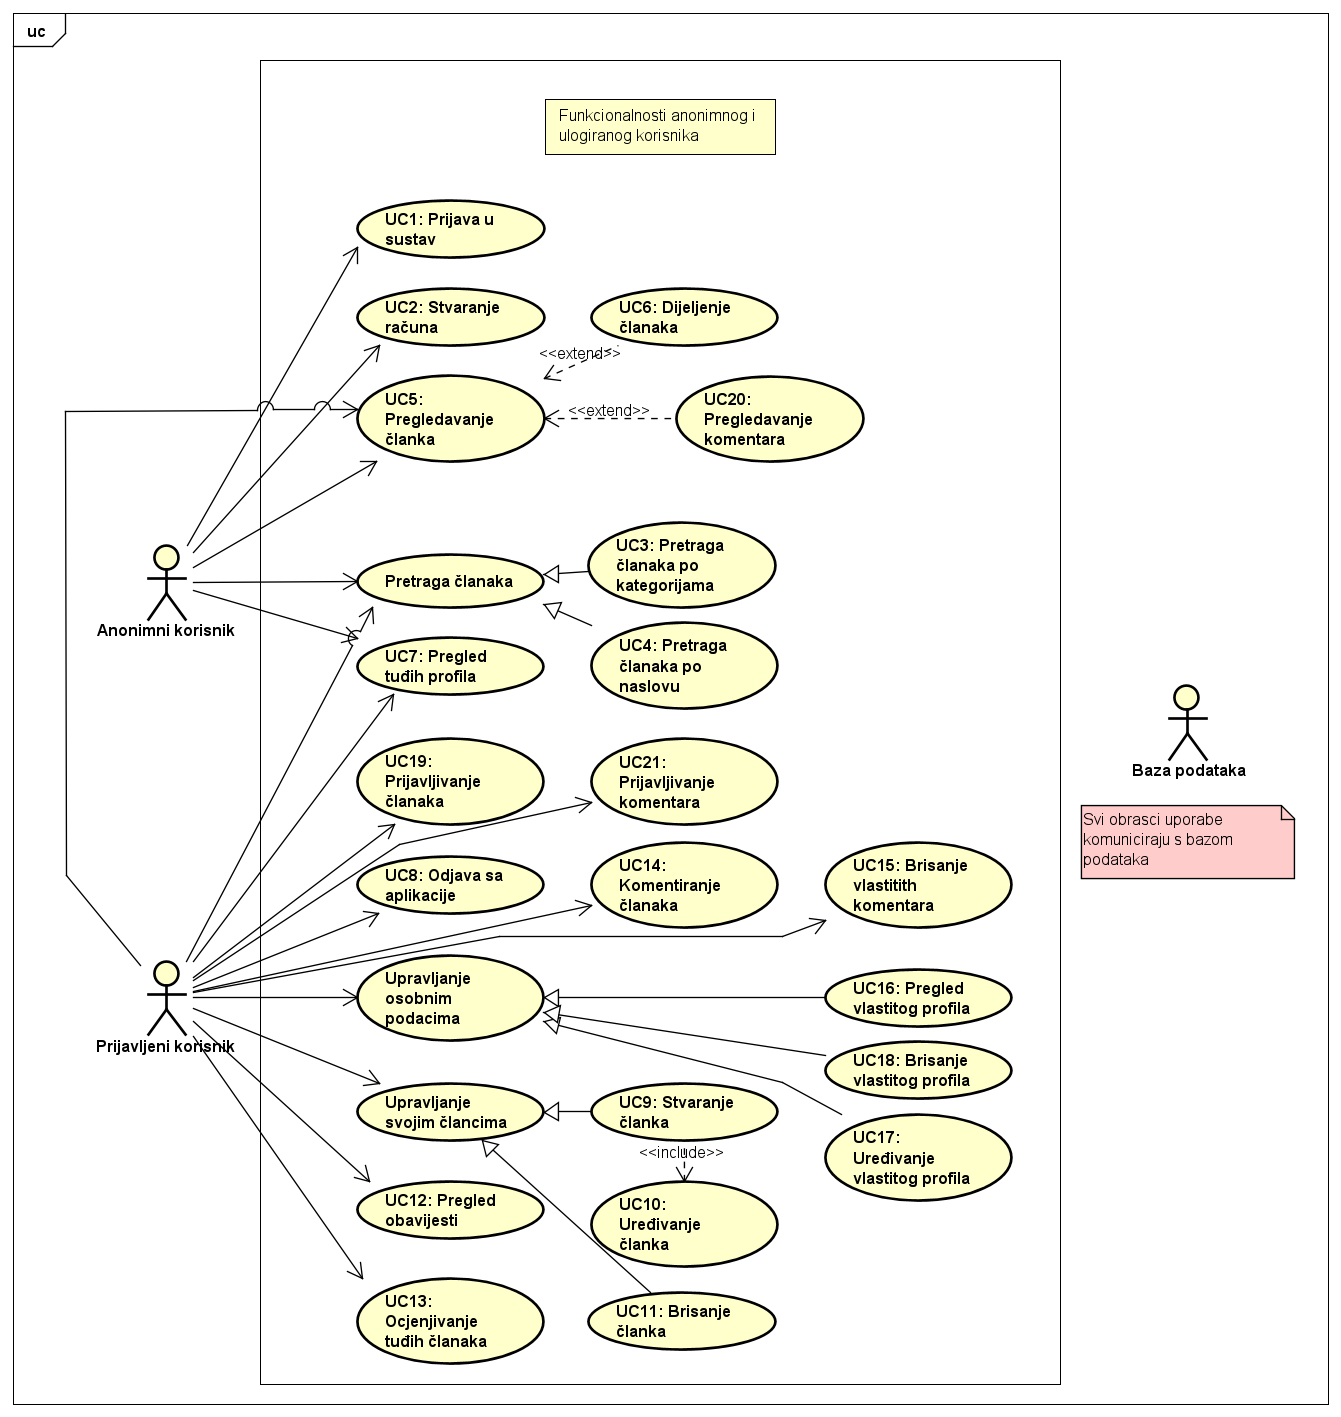
\includegraphics[scale=0.4]{slike/DijagramObrazacaUporabe1.PNG}
	\centering
	\caption{Dijagram obrasca uporabe, funkcionalnost anonimnog i prijavljenog korisnika}
	\label{fig:obrazac_uporabe1}
\end{figure}

\eject		

\begin{figure}[H]
	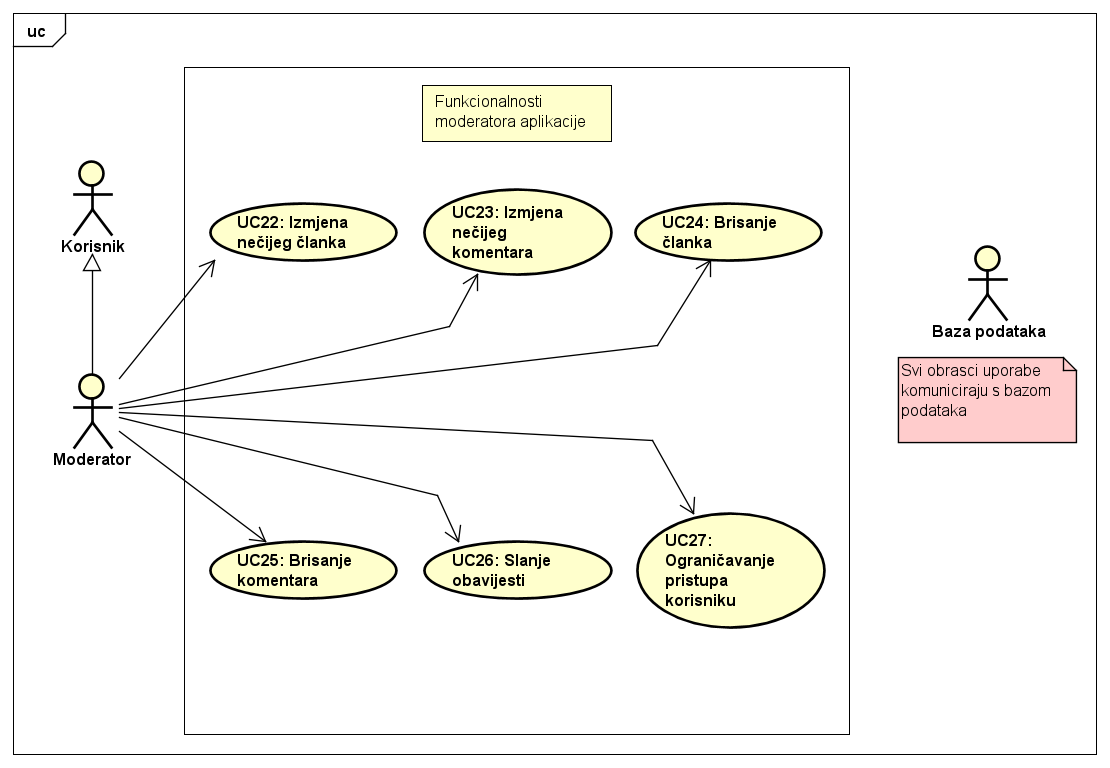
\includegraphics[scale=0.4]{slike/DijagramObrazacaUporabe2.PNG}
	\centering
	\caption{Dijagram obrasca uporabe, funkcionalnost moderatora sustava}
	\label{fig:obrazac_uporabe2}
\end{figure}

\begin{figure}[H]
	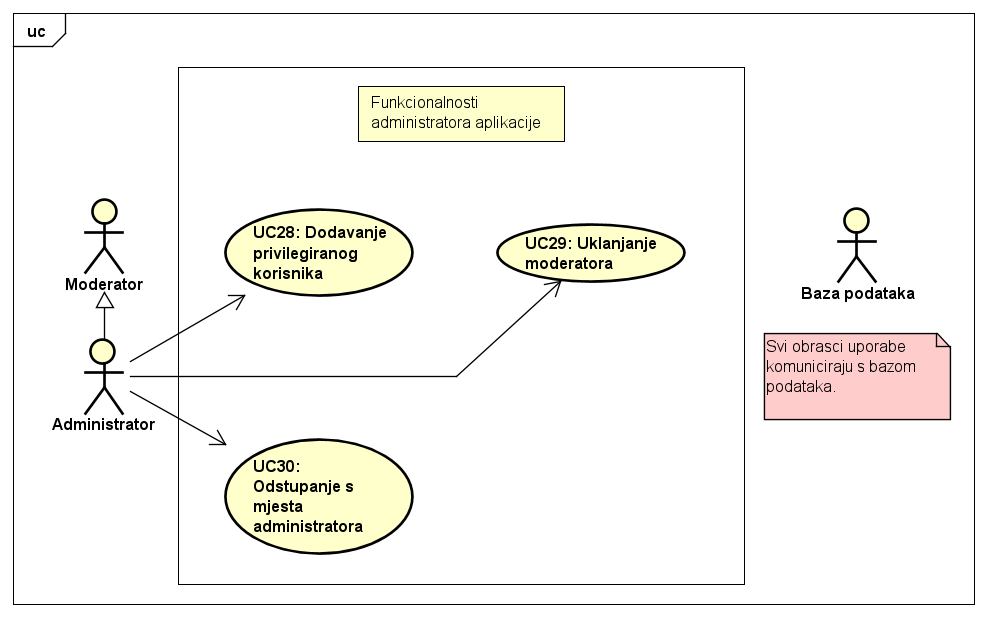
\includegraphics[scale=0.4]{slike/DijagramObrazacaUporabe3.PNG}
	\centering
	\caption{Dijagram obrasca uporabe, funkcionalnost administratora sustava}
	\label{fig:obrazac_uporabe3}
\end{figure}

\eject	

\subsection{Sekvencijski dijagrami}

\textbf{Obrazac uporabe UC3 - Pretraga članaka po kategorijama}

Korisnik šalje zahtjev za prikaz članaka određene kategorije. Poslužitelj dohvaća tražene članke i prikazuje ih.
Ako korisnik zatraži dodavanje određenih filtera, poslužitelj dohvati tražene članke iz prethodno definirane kategorije i prikaže ih.

\begin{figure}[H]
	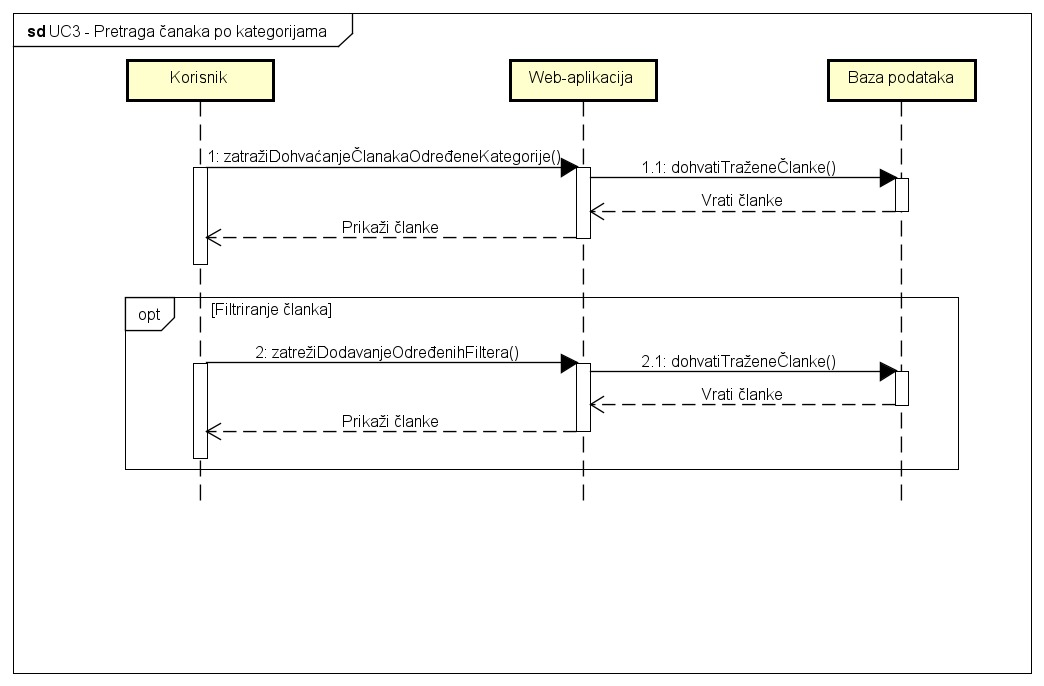
\includegraphics[scale=0.6]{slike/SekvencijskiDijagramUC3.jpg}
	\centering
	\caption{Sekvencijski dijagram za UC3}
	\label{fig:sekvencijski_dijagram_uc3}
\end{figure}

\eject

\textbf{Obrazac uporabe UC9 - Stvaranje članaka}

Korisnik zatraži od aplikacije stvaranje novog članka. Aplikacija prikaže uređivač teksta.
Tijekom uređivanja teksta, korisnik može zatražiti pohranu promjena koje poslužitelj spremi u bazu podataka.
Konačno, korisnik zatraži spremanje i objavu članka. Poslužitelj označi članak kao objavljen, spremi ga u bazu te potvrdi spremanje i objavljivanje.

\begin{figure}[H]
	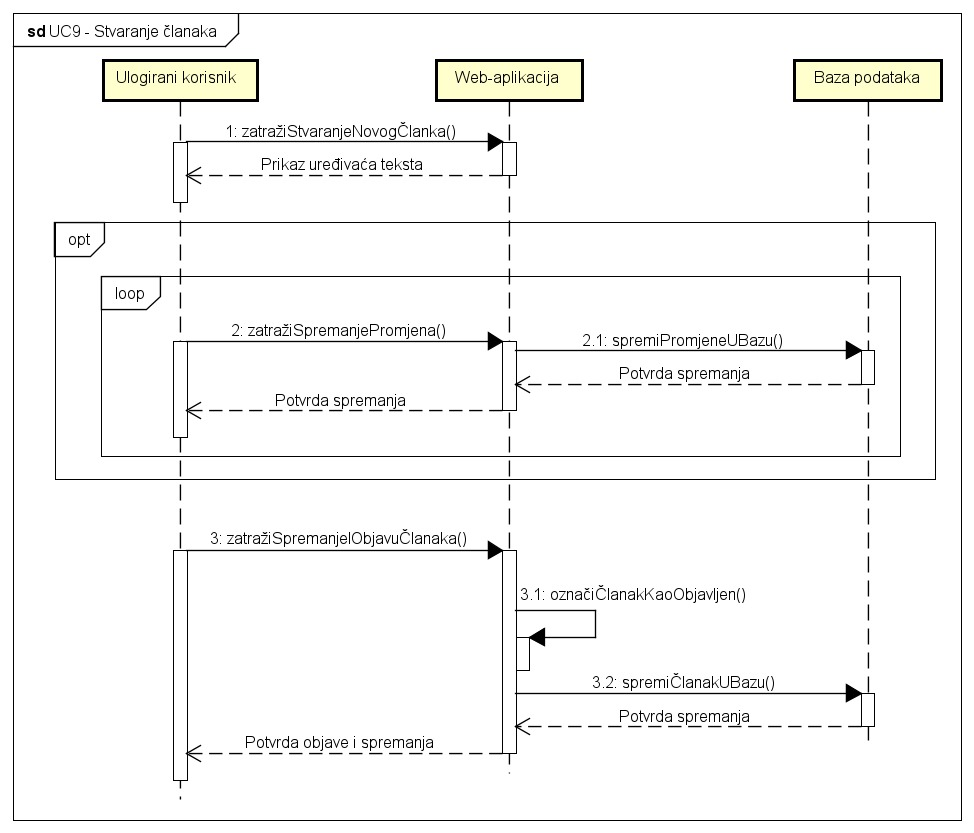
\includegraphics[scale=0.6]{slike/SekvencijskiDijagramUC9.jpg}
	\centering
	\caption{Sekvencijski dijagram za UC9}
	\label{fig:sekvencijski_dijagram_uc9}
\end{figure}

\eject

\textbf{Obrazac uporabe UC14 - Komentiranje članaka}

Korisnik zatraži prikaz članka koji želi komentirati. Poslužitelj dohvati članak iz baze podataka te ga prikaže korisniku zajedno s formom za ostavljanje
komentara. Odabirom forme korisnik zatraži stvaranje komentara za navedeni članak. Poslužitelj prvo dohvati podatke o korisniku kako bih provjerio ima li korisnik
pravo objavljivanja komentara. Ako ima, korisniku se prikaže forma za uređivanje komentara. Nakon napisanog komentara korisnik zatraži njegovu objavu. Ako je komentar
uspješno spremljen, poslužitelj ga spremi u bazu podataka te korisniku potvrdi objavu njegovog komentara. Ako je komentar prazan, korisniku se ispiše poruka da komentar
ne smije biti prazan. Ako se ustanovi da korisnik nema pravo na objavu komentara, odgovarajuća forma se ne prikazuje te se korisniku ispiše odgovarajuća poruka.

\eject

\begin{figure}[H]
	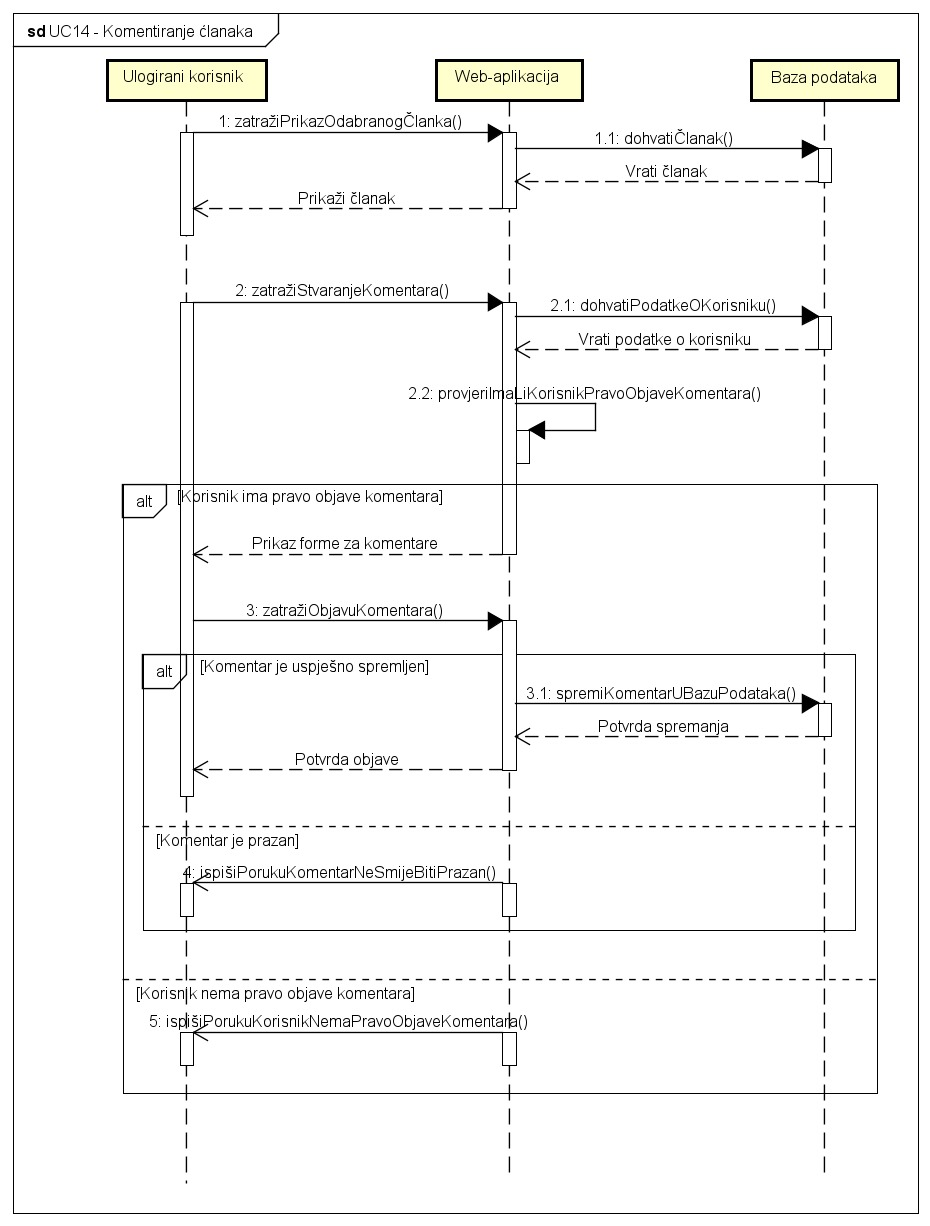
\includegraphics[scale=0.6]{slike/SekvencijskiDijagramUC14.jpg}
	\centering
	\caption{Sekvencijski dijagram za UC14}
	\label{fig:sekvencijski_dijagram_uc14}
\end{figure}

\eject

\textbf{Obrazac uporabe UC26 - Slanje obavijesti}

Moderator zatraži slanje obavijesti (notifikacije) korisniku. Poslužitelj moderatoru prikaže formu za uređivanje obavijesti. Dok nisu uneseni svi primatelji,
moderator unosi primatelje putem forme. Poslužitelj provjerava postoji li navedeni primatelj. Ako postoji, poslužitelj potvrdi moderatoru unos primatelja. U suprotnom slučaju
moderatoru se ispiše upozorenje da navedeni primatelj ne postoji.
Nakon upisivanja primatelja, moderator uređuje sadržaj obavijesti. Nakon što je moderator gotov s uređivanjem, zatraži slanje obavijsti. Poslužitelj provjeri ispravnost unesenih
podataka. Ako su podaci ispravni, poslužitelj spremi obavijest u bazi te istu pošalje svim navedenim primateljima nakon čega potvrdi moderatoru slanje odgovarajuće obavijesti.
Ako podaci nisu ispravni, moderatora se upozori da podaci nisu ispravni. 

\eject

\begin{figure}[H]
	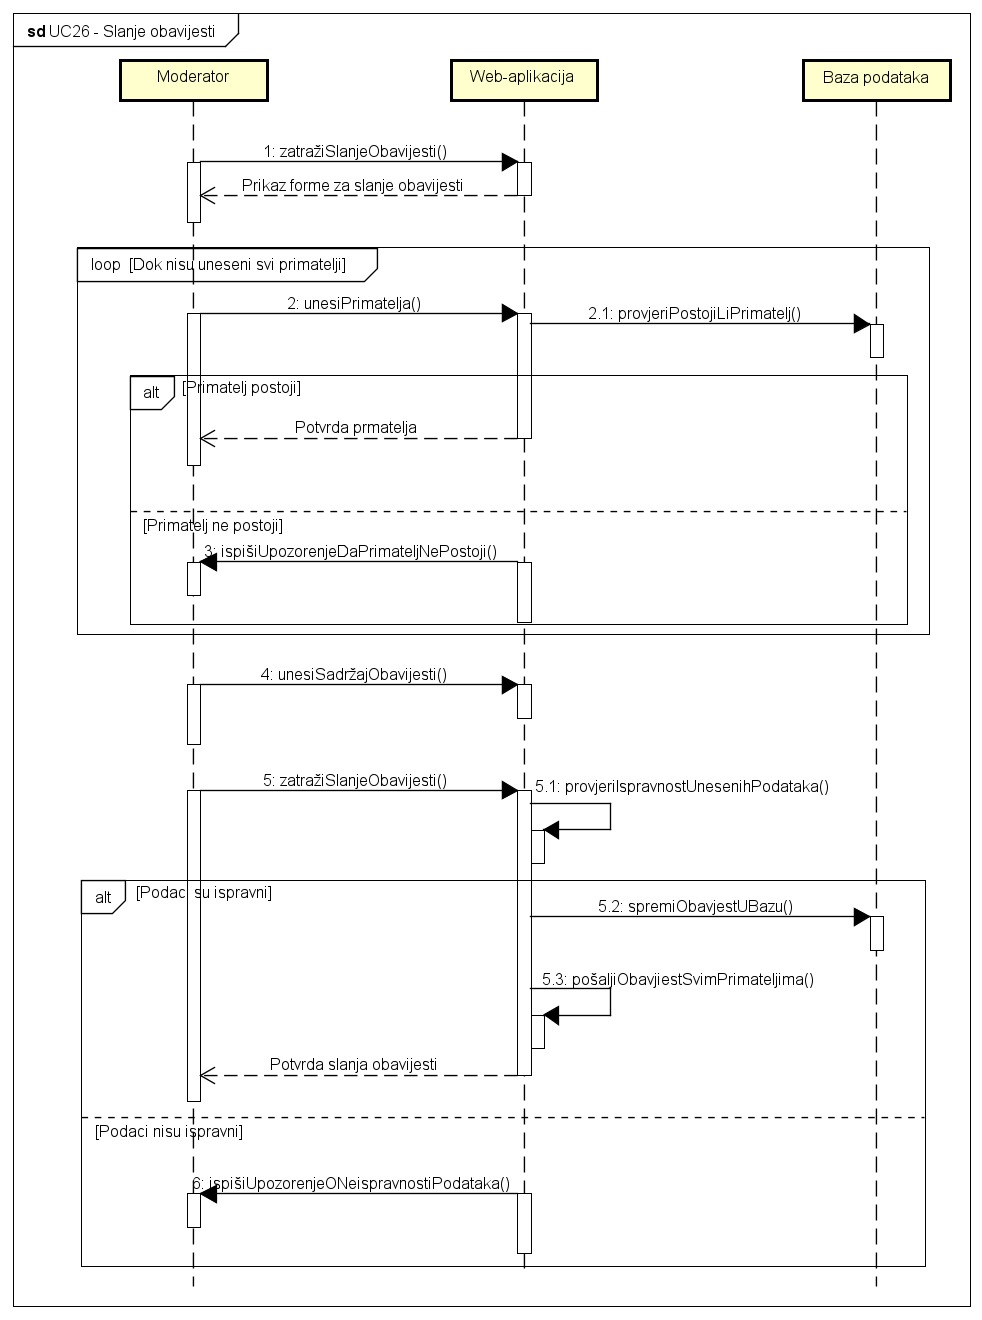
\includegraphics[scale=0.6]{slike/SekvencijskiDijagramUC26.jpg}
	\centering
	\caption{Sekvencijski dijagram za UC26}
	\label{fig:sekvencijski_dijagram_uc26}
\end{figure}

\eject

\section{Ostali zahtjevi}

\begin{enumerate}

    \item Performanse sustava:
        \begin{itemize}
            \item Omogućiti rad više korisnika u stvarnom vremenu
            \item Optimizirati brzinu pristupa bazi podataka
            \item Osigurati učinkovitost interakcije korisnika s platformom
        \end{itemize}

    \item Podrška jeziku i pismu:
        \begin{itemize}
            \item Implementirati podršku hrvatskoj abecedi i dijakritičkim znakovima
        \end{itemize}

    \item Fleksibilnost tehnologije:
        \begin{itemize}
            \item Implementirati InterFER kao web aplikaciju
            \item Koristiti objektno-orijentirane jezike za razvoj
        \end{itemize}

    \item Stabilnost i prilagodljivost:
        \begin{itemize}
            \item Osigurati da nadogradnje ne naruše postojeće funkcionalnosti
            \item Održavati stabilnost sustava tijekom promjena i dodataka
        \end{itemize}

    \item Korisničko iskustvo:
        \begin{itemize}
            \item Osigurati jednostavno i intuitivno korisničko sučelje
            \item Poticati aktivno sudjelovanje korisnika bez potrebe za dugim uputama
        \end{itemize}

    \item Zaštita baze podataka:
        \begin{itemize}
            \item Zaštititi bazu podataka od vanjskih prijetnji
            \item Održavati brzinu i otpornost na vanjske greške
        \end{itemize}

    \item Pristup iz javne mreže:
        \begin{itemize}
            \item Osigurati enkripciju podataka i privatnost korisnika prilikom pristupa izvan zaštićene mreže
        \end{itemize}

\end{enumerate}



